\section{Implementation}
\label{sec:implementation}
	% Chapter concerning the Technical Realization

	In this chapter we will deal with the infrastructure and technical realization of the public display survey platform. First off, we will start with the requirements for the survey platform (section \ref{sec:implementation:requirements}). Subsequently the architecture resulting from the design decisions will be the main focus (section \ref{sec:implementation:design-decisions}). To facilitate the training period for successors we will also take a brief look at the software model (section \ref{sec:implementation:modeling}). For more specific information and for information regarding maintenance of the project, please refer to the Documentation found on the CD enclosed or on the GitHub repository (see Appendix \ref{appendix:documentation}).

	In figure \ref{fig:4-pdsurvey-platform} a brief overview of the \textit{PDSurvey} platform and its components is given. The platform consists of three major parts: a backend for display providers (PDAdmin), a RESTful server (PDServer) and the user interface itself, being embedded on the end user devices (public displays, tablets, smartphones or other devices). 






\subsection{Requirements}
\label{sec:implementation:requirements}

	The starting point for the PDSurvey platform and the Master's thesis itself was the official announcement\footnote{\url{http://www.medien.ifi.lmu.de/lehre/arbeiten/detail.xhtml-php?pub=alt_pdsurvey} (accessed on March 24, 2015)}, describing the scope of the thesis. This problem statement already included first requirements for the survey platform to develop, and was also a trigger for further literature research and talks with people from the industry.

	% Official Problem statement
	\begin{enumerate}[itemsep=0pt] 
	\item development of a survey tool that allows interactive public display installations to be comprehensively assessed 
	\item a web-based survey platform will be implemented that can easily be used to evaluate and compare public displays through different channels 
	\item different channels to support: 1) evaluation directly at
	the display or 2) through a (mobile) website that allows participation also via a smartphone
	or tablet.
	\item configuration options for public display owners
	\end{enumerate}

	Additional requirements, dervived from the previous and complemented with additional ones, are listed below:

	% Derived requirements
	\begin{itemize}[itemsep=0pt] 
	\item easy \textbf{embedding of questionnaires} on websites of public display owners (provide API / embed code)
	\item support of \textbf{various devices}: public displays of all sizes, tablets, phablets, smartphones, desktop devices (responsive web design)
	\item create an \textbf{open research platform} (host project and documentation on GitHub, release it as open source, publish and invite fellow researchers)
	\item allow for both \textbf{quantitative and qualitative} metods of data collection
	\end{itemize}

	% + RESULTS FROM LITERATURE RESEARCH (TODO)

	These derived requirements had an impact on the chosen architecture, which will be discussed in the following.



\subsection{Design Decisions}
\label{sec:implementation:design-decisions}

	After having assessed all requirements for the platform (see section \ref{sec:implementation:requirements}), the next step was making design decisions for the software, programming language and frameworks to use, before starting with the practical implementation of the platform. 

	Two weeks were taken for assessing all of the possibilities, on the one hand to get informed again what is buzzing, on the other hand because every choice also has a significant impact on the later architecture. Changing a technology in between would not be a smart choice in such a short time-frame. 


	\paragraph{Programming language}

		Due to the requirements and objective to support a large number of devices, operating systems, and form factors, a device-independent programming language was preferred. 
		The choice fell on Javascript, not just due to the growing popularity\footnote{\url{http://www.sitepoint.com/javascript-internet-things/} (accessed on November 27, 2014)}, but also because it can be used on the largest number of devices. Furthermore another huge benefit, only having to use JavaScript on all tiers, from client to server to persistence layer.

		This approach has become very popular in recent years, now often being referred to as the MEAN stack, consisting of MongoDB, Express.js, Angular.js, and Node.js. Some fundamental differences to the LAMP stack (Linux, Apache, MySQL, PHP) are its shift form server-side to client-side single-page applications (SPA), faster prototyping, shift from synchronous to asynchronous, fast page loading times, less time spent writing SQL (schemaless), and the shift to using RESTful services for the backend\footnote{\url{http://www.ibm.com/developerworks/library/wa-mean1/index.html} (accessed on March 26, 2015). Additional, the feedback from the industry contacts also played a role. 
		% This already led to the thought of choosing the MEAN stack\footnote{\url{http://mean.io/} (accessed on March 26, 2015)} for the entire development.

		Alternative languages considered were: PHP, Python, Ruby, Java and ASP.NET. The biggest drawback was the additional workload on having to maintain the object model on multiple platforms. With Javascript it is possible to work with the same object model and easily keeping it consistent across all platforms (backend, frontend, server).

		% say because of embedding, it seems obvious to choose JavaScript


	\paragraph{Frontend}

		The next question to be answered was which technologies to use in the frontend, leading to the question whether to follow the single-page application approach or not. As of 2014 the JavaScript model-view frameworks most frequently used for creating single-page apps are Angular.js, Ember.js and Backbone.js. Purely based on numbers Angular.js is the clear favorite, it has by far the largest user base on GitHub, Stackoverflow, and Youtube\footnote{\url{https://www.airpair.com/js/javascript-framework-comparison} (accessed on January 11, 2015)}. When comparing the number of third-party modules, Angular.js also takes the lead with 800 ngmodules vs. 236 Backbone.js backplugs vs. 21 emberaddons. All these factors together indicate a short training time and give hope for making good progress for beginners. These were amongst other things the reasons why we chose Angular.js for this project, since the desired requirement is also for other students to further enhance the PDSurvey platform in the future.

		% Huge benefits for using Angular.js:
			- two-way data-binding, syncing, templating, being able to create your own html-tags with custom directives.

		To speed up frontend development we chose Bootstrap\footnote{\url{http://getbootstrap.com/} (accessed on December 1, 2014)} as our CSS framework of choice. Reasons for choosing Bootstrap were the large community, extensive documentation with helpful examples, large number of free tutorials and templates, its integration with Angular.js (AngulatStrap\footnote{\url{http://mgcrea.github.io/angular-strap/}} and AngularUI), and its short training time.
		Alternatives considered were Foundation Framework by Zurb, however at the time of writing there was no prefabricated integration for Foundation and Angular.js.
		A good overview\footnote{\url{http://www.sitepoint.com/5-most-popular-frontend-frameworks-compared/} (accessed on December 2, 2014)} and a comparison\footnote{\url{http://www.sitepoint.com/grid-system-comparison-bootstrap-vs-foundation/} (accessed March 24, 2015)} of currently popular frontend frameworks was also considered.

		% Express.js was chosen over Resty, simply due to its popularity and because it already suits the MEAN stack philosophy
	


	\paragraph{Backend}

		For the backend it was most important to have a solid and scalable solution with good performance, since our system might need to scale in the future, having a multiplicity of clients attached to the survey platform, all submitting responses and querying for different questionnaires. Additionally an administrator interface and easily being able to exchange data with all clients was of importance. For this reason a backend built solely on the principles of a RESTful API was preferred, being able to use the same data on no matter which platform.

		% get curve to MEAN, say why we chose it now

		Going along with the MEAN stack it was clear to use Node.js as the underlying platform for building web applications. 

		% now it was the question whether to use 
		> give a short overview of alternatives

		 - Express.js
		 - Connect
		 - Koa
		 - Restify


		% Reasons for choosing Node.js
		NodeJS is currently becoming the de-facto standard for scalable and RESTful web services. Another benefit of using Node.js being easily able to implement authentication or internationalization of the whole platform through the concept of the middlewares \footnote{\url{http://www.heise.de/developer/artikel/REST-Webservices-mit-Node-js-Teil-1-Connect-als-Fundament-1802258.html?view=print} (accessed on November 24, 2014)}. 

			\begin{enumerate}[itemsep=0pt] 
			\item scalable
			\item modular / extensible
			\item multilingual / internationalization (i18n)

	        \item \textbf{Backend}: Why I chose Node.js
	        \item Frameworks in Node.js: Connect, Express, Koa, ... which ones I chose why
	        \item Discussion of pro/con Node.js: http://www.heise.de/developer/artikel/2x-Nein-4x-Ja-Szenarien-fuer-Node-js-2111050.html
			\end{enumerate}


		% Choosing Object Model ... Layer
		Mongoose.js\footnote{\url{http://mongoosejs.com/} (accessed on November 14, 2014)}



		% + Interaction / Communication
	
		> REST vs SOAP: why I chose REST

		Should a component not support HTML or JavaScript execution, then the required surveys can still be communicated directly with the REST API through rudimentary HTTP function calls.

		Based on these requirements and the feedback received from industry experts, a choice towards Node.js and to fully go along with MEAN stack was self-evident.




	\paragraph{Database}

		Another fundamental aspect presented the question where to store the data persistently. Criteria for choosing the right database management system (DBMS) for this project were again the size of community, suitability for prototyping, and ease of integration with Node.js/Angular.js.

		The first question presented whether to choose a SQL or a NoSQL DBMS. Because NoSQL is better for rapid prototyping, its Schema can be mixed inside of one collection and develop over time. Combined with the benefit of having a better scalability, a schemaless data representation, faster response time and a decreased development time\cite{vaish2013getting}, these are all reasons speaking for using a NoSQL DBMS for our scenario. 

		Out of the NoSQL databases MondoDB\footnote{\url{http://www.mongodb.org/}} represents the most popular DBMS, especially since it integrates seamlessly into the MEAN stack. With the help of Mongoose\footnote{\url{http://mongoosejs.com/} (accessed November 14, 2014)}, a object modeling package for Node.js, performing CRUD applications on MongoDB and maintaining a solid object model (schema) gets even easier.


		Benefits of MongoDB are being non-relational (and schemaless), plus its ability to directly store JavaScript object inside the database, being the biggest advantage. One disadvantage is that MongoDB does not support joins or transactions. For our use case, however, this is no major drawback. The benefits outweigh the disadvantages.

			% Reasons for using MongoDB
			% \begin{enumerate}
			% \item ideal for lots of write procedures
			% \item non-blocking write operations, ideal for Node.js and for logging data (good for our future work)
			% \item good read performance
			% \item good scalability
			% \item fully supports JSON syntax
			% \item good integration with Node.js, see Mongoose\footnote{http://mongoosejs.com/}
			% \end{enumerate}

			% Notes from the MondoDB University M101JS Class
			% \begin{enumerate}
			% \item is non-relational, ideal for JSON data
			% \item MongoDB is schemaless. Two documents in the same collection can have different schemas.
			% \item MongoDB provides a good compromise between scalability/performance and the depth of funcitonality
			% \item Drawback: MongoDB does not support Joins or Transactions
			% \end{enumerate}


		Alternatives looked at were CouchDB and Redis\footnote{\url{http://kkovacs.eu/cassandra-vs-mongodb-vs-couchdb-vs-redis} (accessed March 26, 2015)}. Redis being useful for fast changing data, which is not the case for our platform. CouchDB would be an alternative worth looking at, having a better replication and conflict resolution. This additional securitry is however not needed. The speed benefits of MongoDB, also being able to make dynamic queries, are preferred.





	\paragraph{Hosting}

		For the hosting of the platform a free and easy scalable solution was of importance. Our first choice was Heroku\footnote{https://www.heroku.com/}, due to its simplicity of setup, its native support of Node.js and the seamless integration with Mongolab\footnote{https://mongolab.com/}, hosting our MongoDB.

		% TODO: IaaS vs PaaS: https://www.youtube.com/watch?v=Q8jZHc0NS6A
		% give reasons why I chose PaaS (Platform as a Service)

		    % Heroku        PaaS
		    % IBM BlueMix   PaaS
		    % Amawon AWS    IaaS
		    % self hosting  IaaS

		    %   comparison  http://smashingboxes.com/ideas/heroku-vs-amazon-web-services


		Alternative were Google App Engine, IBM BlueMix, Amazon Web Services (Amazon EC2) or hosting everything on local or virtualized machines at our university. However for our scenario all of the above options had their drawbacks in comparison to Heroku. Google App Engine (as of December 2014) still had no native support for Node.js and custom runtimes had to be used to get Node.js support up and running. IBM BlueMix just got overhauled, offered full out-of-the-box Node.js support, however they only the first 30 days were free and the pricing model wasn't as attractive. Amazon Web Services offering a Infrastructure as a Service (IaaS), would have required too much administration of the server, which would have slowed down the main objective of the project, the development of the survey platform. The same goes for the last option, hosting a MEAN-stack environment on our own servers at LMU Munich. All of the above are well-known solutions in the industry, however due to simplicity and ease of use we chose Heroku.


		\paragraph{MEAN (maybe here)}
			In the end, as already predicted in the beginning, it turned out to be the classic MEAN stack. 

			The clear benefit, being able to use JavaScript from client to server to persistence level. 

			% give further reasons

			+ a fantastic short recap of the the last ten years of web development with an introduction to the MEAN stack, also explaining what the differences are between traditional web development (using the LAMP stack), to using the MEAN stack:
			\url{http://www.ibm.com/developerworks/library/wa-mean1/index.html} (accessed on March 26, 2015)



\clearpage
\subsection{Modeling}
\label{4c_modeling}

	The model for the \textit{PDSurvey} platform is maintained with the help of the Node package Mongoose. Node.js maps the route parameters and routes all requests to the corresponding Mongoose model. Angular.js builds its model upon the REST API and maps it via dynamic two-way-binding to it's scope. Thus all changes to the model originate from Mongoose.



\subsubsection{Development Process / Modeling}

	The development process of the PDSurvey platform was inspired and influenced by the following approaches:

	\begin{itemize}
	\item working agile and user centered... TODO: look up how to best explain it.

	\item User Centered Design: (paper nr 31): ``constitutes an iterative process of system design, deployment and evaluation'' (quote from paper 31). Work iteratively, continuous deployment and evaluation.

	\item Concept of extreme programming\footnote{\url{http://www.extremeprogramming.org/rules.html} (accessed on November 14, 2014)}: First user stories were written and assessed in a small group. The next step was to transfer these stories to user models, describing in detail which functionality the stakeholders of PDSurvey are supposed to have. Later a first software architecture and software model was built, getting more specific. Dependencies between models were defined and this model was continuously refined and improved throughout the dvelopment phase. The last step of the modeling represented screen designs, getting a clear view of what the interface might later look like.

	\item Used the extreme programming\footnote{\url{http://www.extremeprogramming.org/rules.html} (accessed on November 13, 2014)} approach: user stories, release planning, release schedule, small releases, iterating


	\item criteria for good user stories: http://tigertechtalk.wordpress.com/2012/10/17/wie-schreibe-ich-eine-gute-user-story-und-was-ist-das-uberhaupt/
	\end{itemize}








\subsubsection{User roles}

As of now only two roles are implemented, the admin-role and the guest-role.

% FEEDBACK VON FLORIAN: nein, nicht zu komplex machen. Es sollte sogar reichen, nur zwischen Admin & Operator (= Application Provider) zu unterscheiden, da der end user (das Public Display) ja sowieso nur auf die öffentlichen REST API Zugriff hat. (2014-11-14)


In the long term it would be desirable to have the following user roles: Admin, Operator, Evaluator, DisplayApplication.






\subsubsection{Software model}

In total there are the following classes.

\begin{enumerate}
\item list all classes
\item 1 UML diagram is enough, according to Florian
\end{enumerate}


\subsubsection{Dependencies}

Of special interest are the following four models: Survey, Display, Campaign and Responses.

\paragraph{Surveys:} Surveys resembles the foundation of PDSurvey, with the aim of reuse and standardization. A survey consists of multiple sections, being built of of multiple questions. Each question is of a corresponding question type and every survey belongs to a category. This allows the filtering for relevant surveys. To be able to create private surveys, not being shared across the entire platform, every survey is assigned to an individual user.

\paragraph{Displays:} In the display collection all displays connected to the PDSurvey platform are contained. To allow for an evaluation across multiple display models and based on the context of the displays, the display model and a static and/or dynamic context is assigned to every display.

\paragraph{Campaigns:} Campaigns resemble the most integral part, since they glue all of the pieces together and allow the distribution of surveys to public display networks. A campaign consists of displays and surveys and creates the mapping of the questionnaires to public displays. Additionally to each of those mapping an individual context can be assigned, enabling the later comparison of results in between the public displays.

\paragraph{Responses:} All responses made to each survey are logged in the Response collection. The queries are carried out individually per user, per display and per campaign. This model will be the base for further extensions, amongst others the automatic evaluation of the survey responses and the comparison inbetween an entire display network, to be able to find out which properties of a display might be related to certain effects.

\paragraph{Context:} One of the benefits of creating such a survey platform is being able to collect and evaluate large amounts of data, without having to pay more people for conducting and evaluating the survey. The idea would be to collect a large number of responses from a variety of displays in various settings, and assigning a specific context to every display connected to PDSurvey. Once enough data is collected, having the ability to evaluate and compare the displays between each other. Interesting questions for analysis would be, which role the context plays on how the users behave, when running identical software settings on the displays, but only varying the context (position, size of display, surrounding environment of the display, positioning it outdoors or indoors, influence of the weather, type of building it is positioned in).


\begin{figure}%[btph]
    \begin{center}
        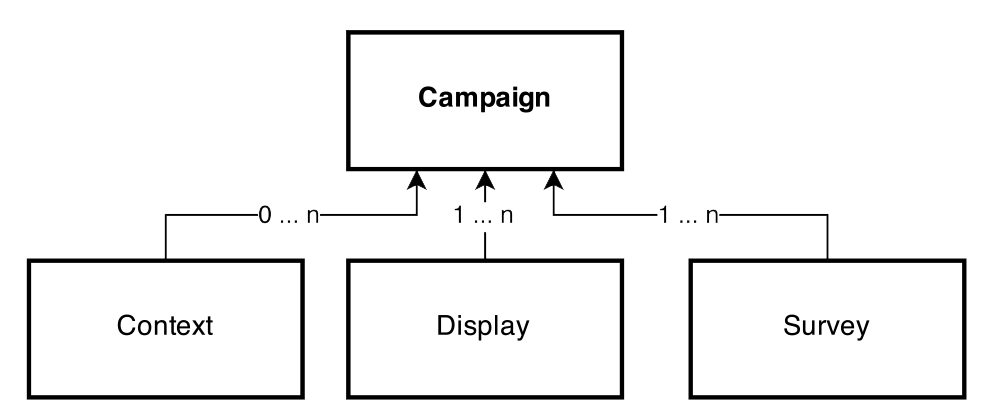
\includegraphics[width=.8\columnwidth]{img/4_implementation/4-dependency-campaign}
    \end{center}
 % \begin{center}\LARGE [BILD]\end{center}
 \caption{Campaign model dependencies}
 \label{fig:4-dependency-campaign}
\end{figure}


++ neue Namensgebung, um in der domain specific language zu bleiben --> application provider / display provider / space provider (anstatt Operator). Wir werden aber nur mit dem Application Provider (anstatt Operator) im System arbeiten





\subsubsection{REST interface}

Defining the REST API. 

% TODO: Explain why I chose which level of separation / detail.

Notes from before I started writing: 
\begin{enumerate}
\item Think about using a Extreme Programming approach http://www.extremeprogramming.org/rules.html
\end{enumerate}
\label{sec:implementation:modeling}

Modeling
	Software Model
	+ Dependencies in between them
	Users
	User Stories
	REST API


Used the extreme programming\footnote{\url{http://www.extremeprogramming.org/rules.html} (accessed on November 13, 2014)} approach: user stories, release planning, release schedule, small releases, iterating


